\documentclass[11pt]{beamer}
\usetheme{CambridgeUS}
%\usepackage[utf8]{inputenc}
%\usepackage[turkish]{babel}
\usepackage{amsmath}
\usepackage{amsfonts}
\usepackage{amssymb}
\usepackage{graphicx}
\usepackage{listings}

\author{Prof.Dr.Mehmet Hakan Satman \\ mhsatman@istanbul.edu.tr}
\title{Scientific Computing and (Big) Data Analysis with Julia}
\setbeamercovered{transparent} 
%\setbeamertemplate{navigation symbols}{} 
\logo{
\includegraphics[width=1cm]{images/iulogo.jpg}} 
\institute{Istanbul University} 
\date{2023.12.01} 

\begin{document}

\begin{frame}

\includegraphics[width=1cm]{images/julia.png}
\titlepage
\end{frame}


\begin{frame}[fragile]{Julia Programming Language}{First things first!}
\begin{lstlisting}
println("Hello, world")
\end{lstlisting}
\end{frame}


\begin{frame}[fragile]{Julia Programming Language}{Welcome!}
	\begin{center}
			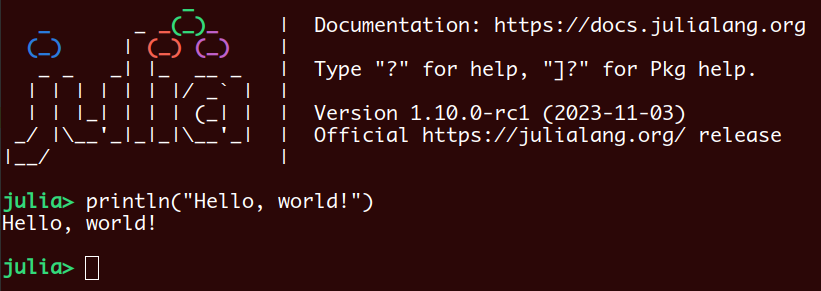
\includegraphics[width=10cm]{images/welcome.png}
	\end{center}
\end{frame}


\begin{frame}[fragile]{Julia Programming Language}{The editor: Visual Studio Code}
	\begin{center}
		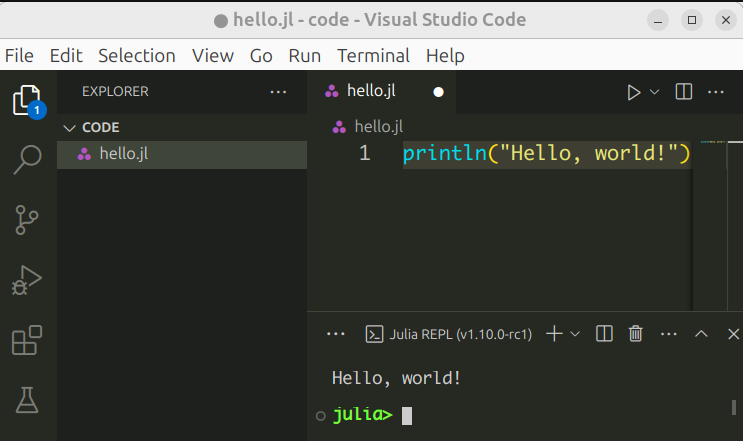
\includegraphics[width=10cm]{images/vscode.png}
	\end{center}
\end{frame}


\begin{frame}[fragile]{XOR}{eXclusive OR}
\begin{table}
\centering
\begin{tabular}{|c|c|c|}
	\hline
	$x_1$ & $x_2$ & $y$ \\
	\hline 
	1 & 1 & 0 \\
	\hline 
	1 & 0 & 1 \\
	\hline 
	0 & 1 & 1 \\
	\hline 
	0 & 0 & 0 \\
	\hline 
\end{tabular}
\caption{$y = \text{xor}(x_1, x_2)$}
\end{table}
\end{frame}

\begin{frame}[fragile]{Symbolic Regression}
	\begin{lstlisting}
using SymbolicRegression, MLJ

x = (
	x1 = Float64[1, 1, 0, 0], 
	x2 = Float64[1, 0, 1, 0]
)
y = Float64[0, 1, 1, 0]

model = SRRegressor(
	niterations = 50,
	binary_operators = [+, -, *],
	unary_operators = [abs],
	should_simplify = true,
	save_to_file = false)

\end{lstlisting}
\end{frame}

\begin{frame}[fragile]{Symbolic Regression}
\begin{lstlisting}
mach = machine(model, x, y)
fit!(mach)
report(mach)
@info predict(mach, x)
\end{lstlisting}
\end{frame}


\begin{frame}[fragile]{Symbolic Regression}
\begin{lstlisting}
Hall of Fame:                                                                                                                                            -------------------------------------------------------------------------------------------------------------------------------------------------------- Complexity  Loss       Score     Equation                                                                                                                1           2.500e-01  3.604e+01  y = 0.5                                                                                                                4           0.000e+00  1.201e+01  y = abs(x1 - x2)                                                                                                       --------------------------------------------------------------------------------------------------------------------------------------------------------
[ Info: [0.0, 1.0, 1.0, 0.0]

\end{lstlisting}
\end{frame}




\end{document}